% !TeX root = ../b01.tex

\section{Aufgabe BI-3}

\begin{task}
    Die folgende Graphik zeigt für $n=200$ Beobachtungen eines Merkmals $X$ die empirische Verteilungsfunktion:

    \begin{figure}[H]
        \begin{center}
            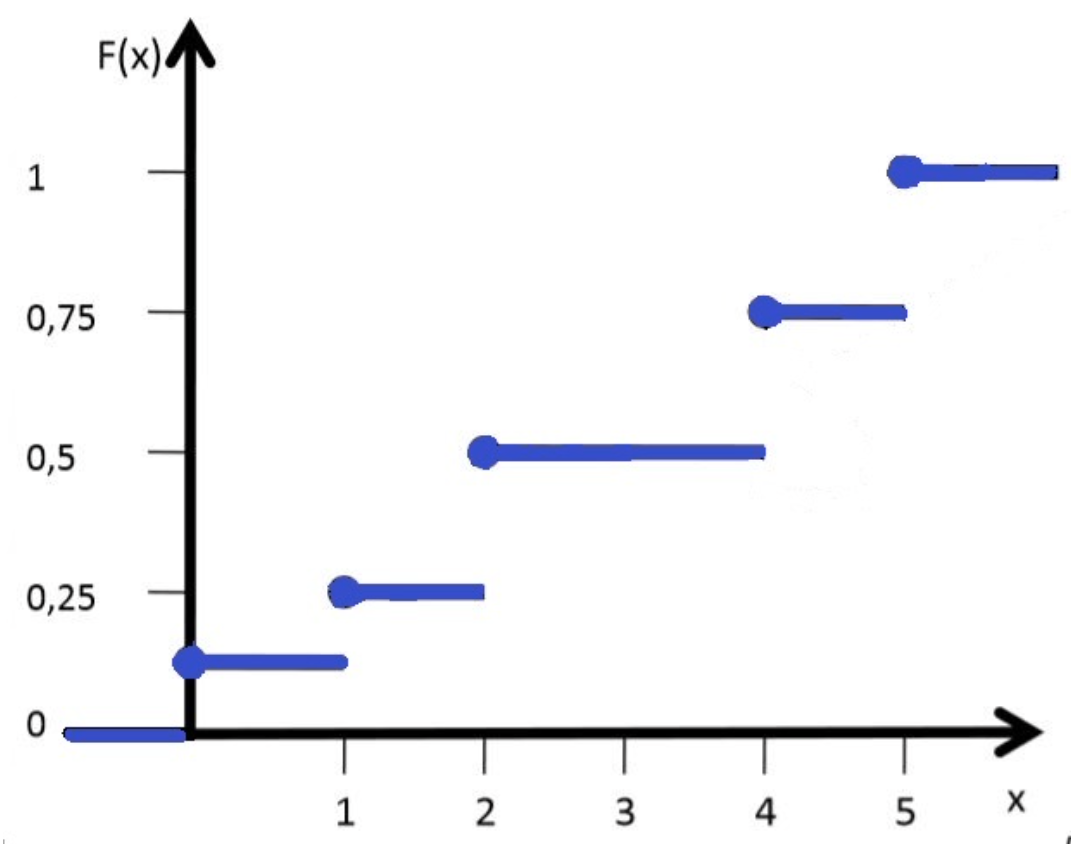
\includegraphics[width=0.3\textwidth]{assets/task3.png}
        \end{center}
    \end{figure}

    \begin{enumerate}
        \item[(a)] Welche Merkmalsausprägungen (verschieden, positiv) wurden für $X$ beobachtet?
    \end{enumerate}
\end{task}

\begin{task}
    \begin{enumerate}
        \item[(b)] Bestimmen Sie die absoluten Häufigkeiten der Merkmalsausprägungen von $X$.
    \end{enumerate}
\end{task}

\begin{task}
    \begin{enumerate}
        \item[(c)] Berechnen Sie das arithmetische Mittel $\overline{x}$ sowie die (korrigierte) Varianz $s^2$ der Daten.
    \end{enumerate}
\end{task}

\begin{task}
    \begin{enumerate}
        \item[(d)] Es wird eine Stichprobe mit zehn weiteren Beobachtungen erhoben. Alle zehn Beobachtungen haben den Wert $3$. Wie lauten dann die neuen relativen Häufigkeiten der Merkmalsausprägungen von $X$ für die um jene Beobachtungswerte erweiterte Stichprobe?
    \end{enumerate}
\end{task}
